\section{Schaltpläne}

Zur Umsetzung des Datenbusses wird für jedes Modul ein Mikrocontroller zur Kommunikation benötigt. 
Über die Mikrocontroller werden die zu verarbeitenden Eingangssignale vom jeweiligen Modul über den Bus an das Controller Modul übertragen. Für die 
unterschiedlichen Funktionen der Module müssen jeweils eigene Platinen entwickelt werden. 


\subsection{Controller Modul}
Der verwendete ESP32 ist wie in Abb. \ref{ESP} verschaltet. Das UART-Bridge wird an den Pins D34 und D35 angeschlossen, da diese al UART Pins vom ESP32 vorgesehen sind. Der interne Datenbus wird an den Pins D13 und D15 angeschlossen, wobei D13 als Receive-Pin und D15 als Transmit-Pin fungiert. Der ESP32 wird über V\textsubscript{in} mit 5V über die USB Spannung versorgt.

\begin{figure}[H]
    \centering    
    \fbox{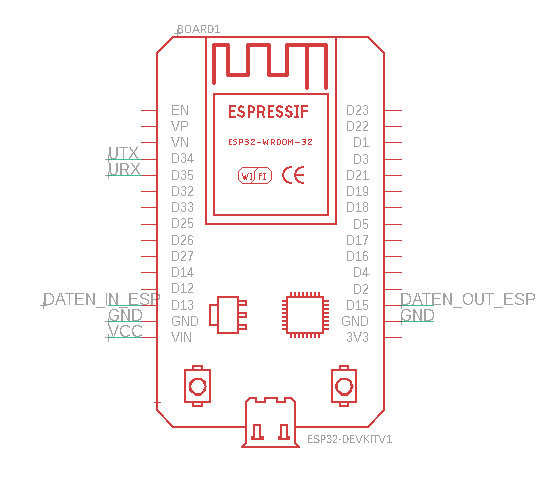
\includegraphics[width=.75\textwidth]{Bilder/ESP.PNG}}
    \caption{ESP32 Verschaltung}
    \label{ESP}
\end{figure}

Für die Kommunikation mit einem PC, werden die Daten über ein UART-Bridge gegeben, bevor sie an die USB Schnittstelle übertragen werden. D+ und D- sind in diesem Fall die USB-Datenleitungen, welche über eine USB-Buchse herausgeführt werden. Die UART-Datenleitungen vom ESP32 zum UART-Bridge sind in Abb. \ref{USB} verdreht, da es sich um die Labels aus Sicht des ESP32 handelt.


\begin{figure}[H]
    \centering    
    \fbox{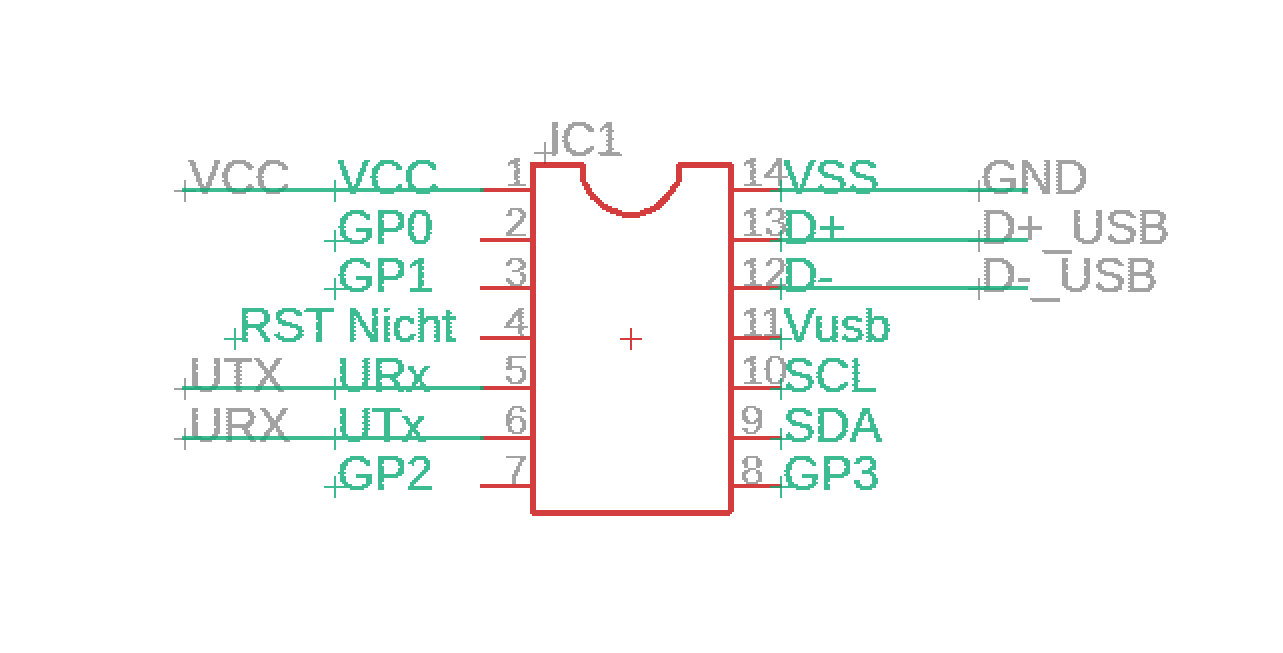
\includegraphics[width=.8\textwidth]{Bilder/BU_USB.PNG}}
    \caption{UART-Bridge}
    \label{USB}
\end{figure}

Zur Kommunikation auf unserem Datenbus werden die Daten differenziell übertragen. Welches über den Transmitter SN65LVS1D und den Receiver SN65LVDT2D passiert.

\begin{figure}[H]
    \centering    
    \fbox{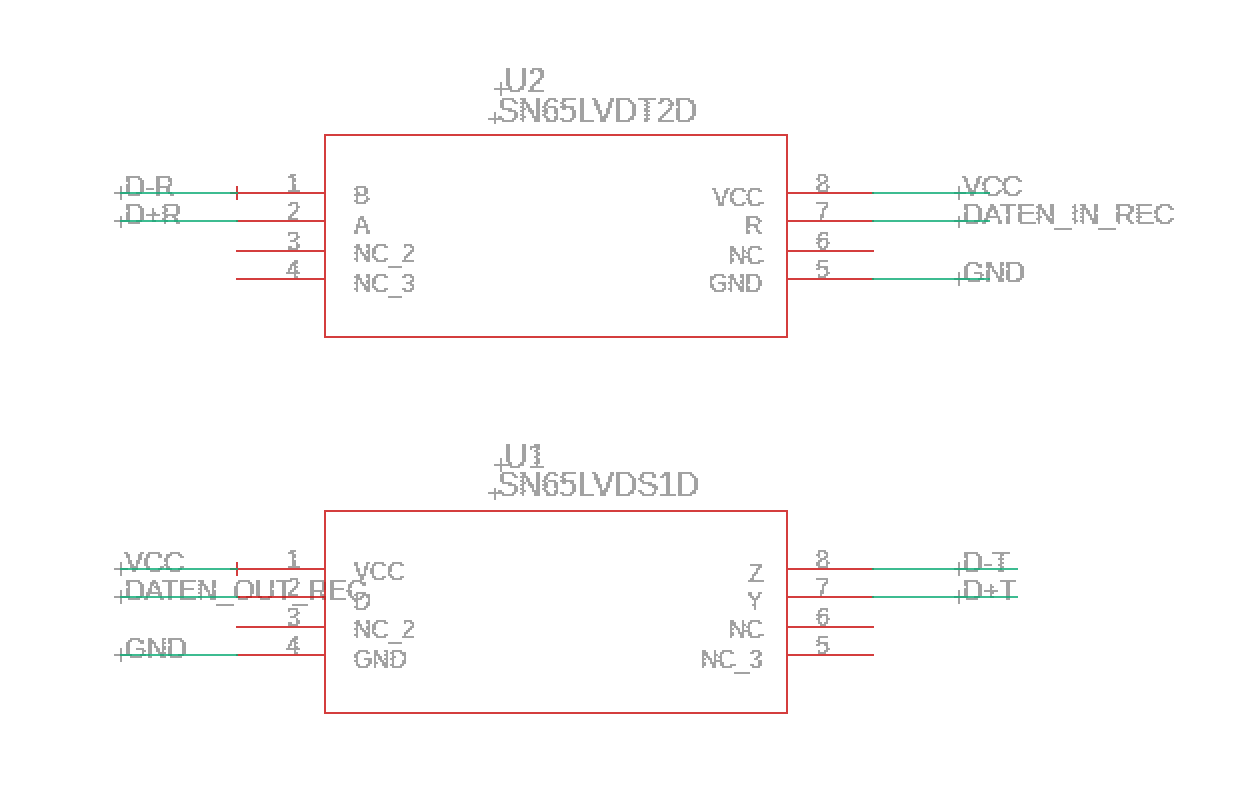
\includegraphics[width=.8\textwidth]{Bilder/BU_T_R_Bausteine.PNG}}
    \caption{Transmit-(SN65LVS1D) und Receiver(SN65LVDT2D) Bausteine }
    \label{T_R_Bausteine}
\end{figure}

\subsection{Tastatur-Modul}
Das Tastatur-Modul besteht aus 4x4 Tasten, die, wie in Abb. \ref{Tastatur} zu sehen, in einer Matrix verschaltet sind. Über die vier Ausgänge (PD2, PD3, PD4, PD5) des  ATmega werden nacheinander 
Ausgangssignale gegeben, während über die vier Eingänge (PD6, PD7, PB0, PB1) die Spalten abgefragt werden. Die Verschaltung des ATmega ist in Abb. \ref{AtMega} zu sehen. Um das korrekte Auslesen mehrerer gedrückten Tasten zu gewährleisten, werden in jedem 
Ausgangspfad Schaltdioden eingesetzt. \\
Die Datenübertragung findet über die Pins PD0 und PD1 statt.


\begin{figure}[H]
    \centering    
    \fbox{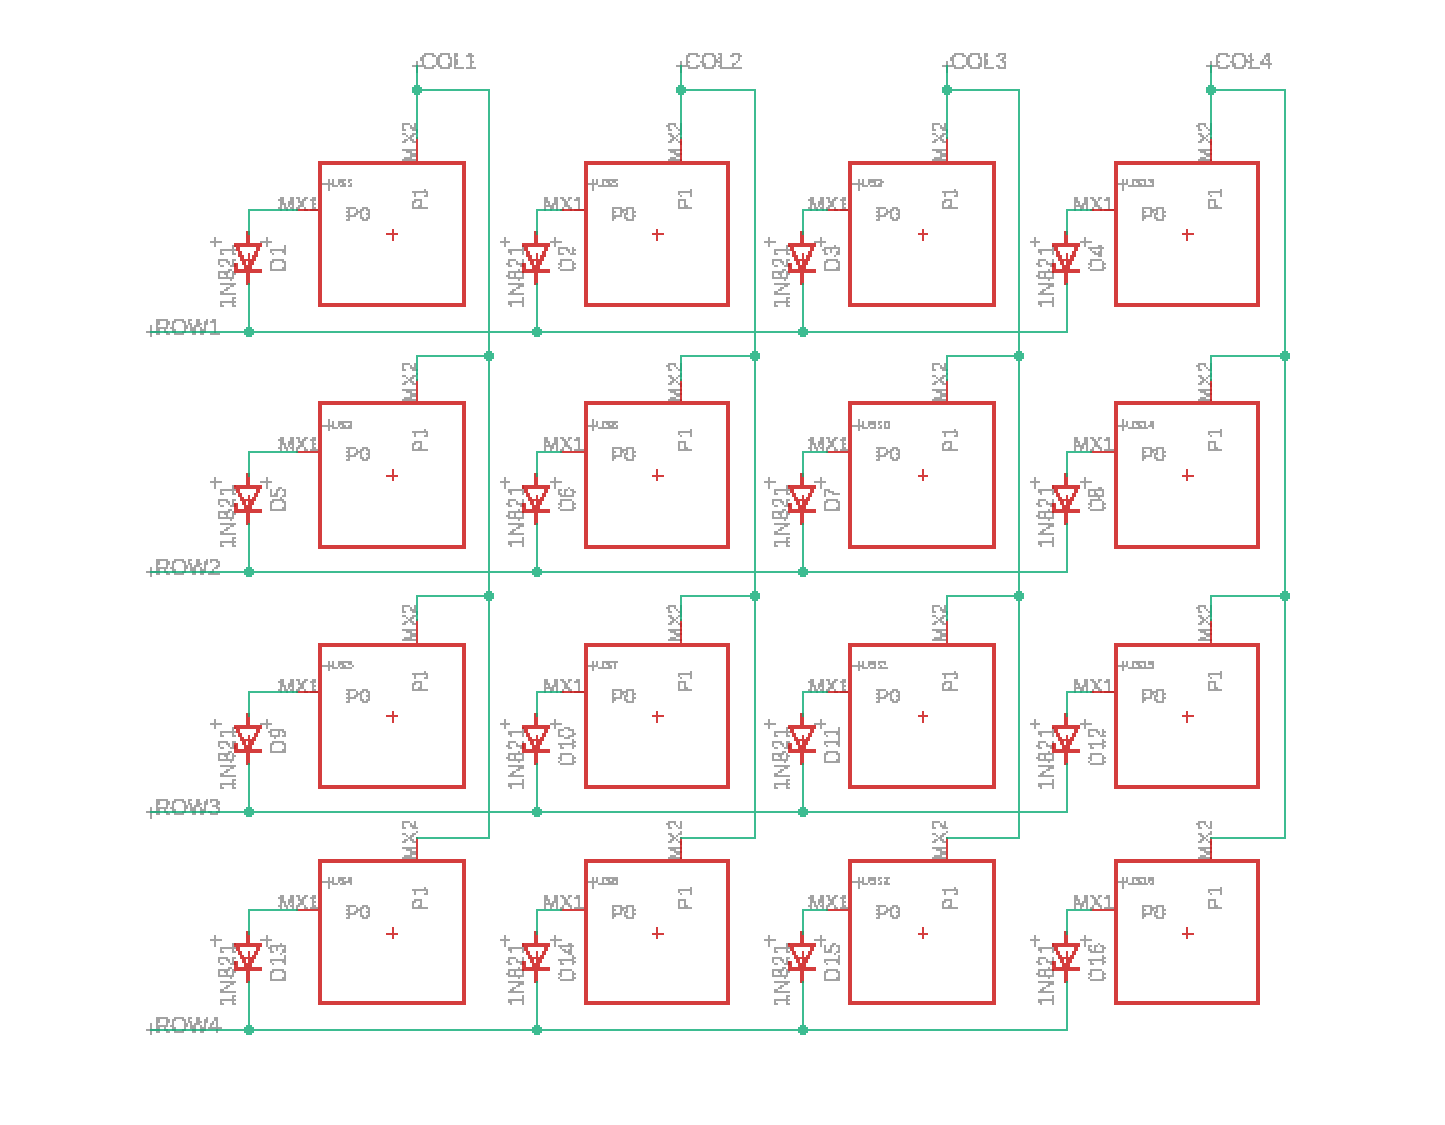
\includegraphics[width=1\textwidth]{Bilder/BU_Tastatur.PNG}}
    \caption{Tastatur Schaltung}
    \label{Tastatur}
\end{figure}


\begin{figure}[H]
    \centering    
    \fbox{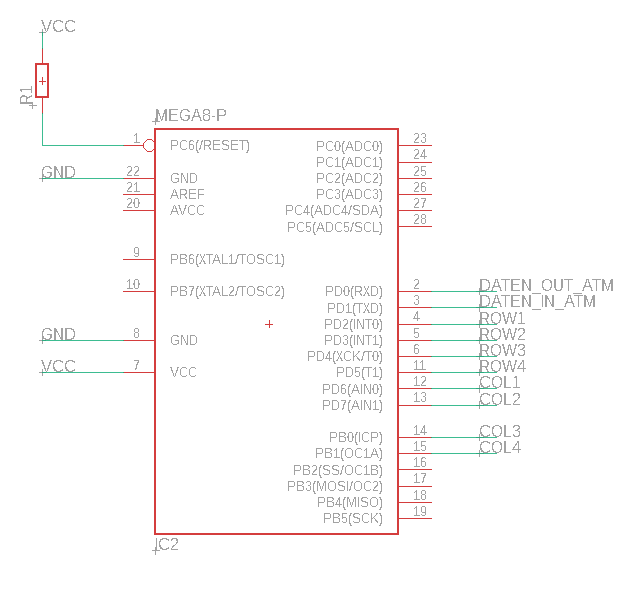
\includegraphics[width=.85\textwidth]{Bilder/AtMega.PNG}}
    \caption{ATmega Verschaltung}
    \label{AtMega}
\end{figure}


\subsection{Alternativen zum Transceiver}

Aufgrund der Probleme bei der Realisierung wurde sich dazu entschieden auf dem PCB mehrere Möglichkeiten zur differenziellen Übertragung vorzusehen 
und über Jumper schalten zu können. 
Es wird die folgenden Möglichkeiten geben:

\begin{itemize}
\item nur die Transmit/Receive ICs zu verwenden,
\item die Transmit/Receive ICs mit zusätzlichen Optokopplern zu verwenden,
\item die Optokoppler mit diskret aufgebautem Invertierern und
\item das Umschalten auf eine Lochrasterplatine, andere Testschaltungen/Testbausteine
\end{itemize}



\begin{figure}[H]
    \centering    
    \fbox{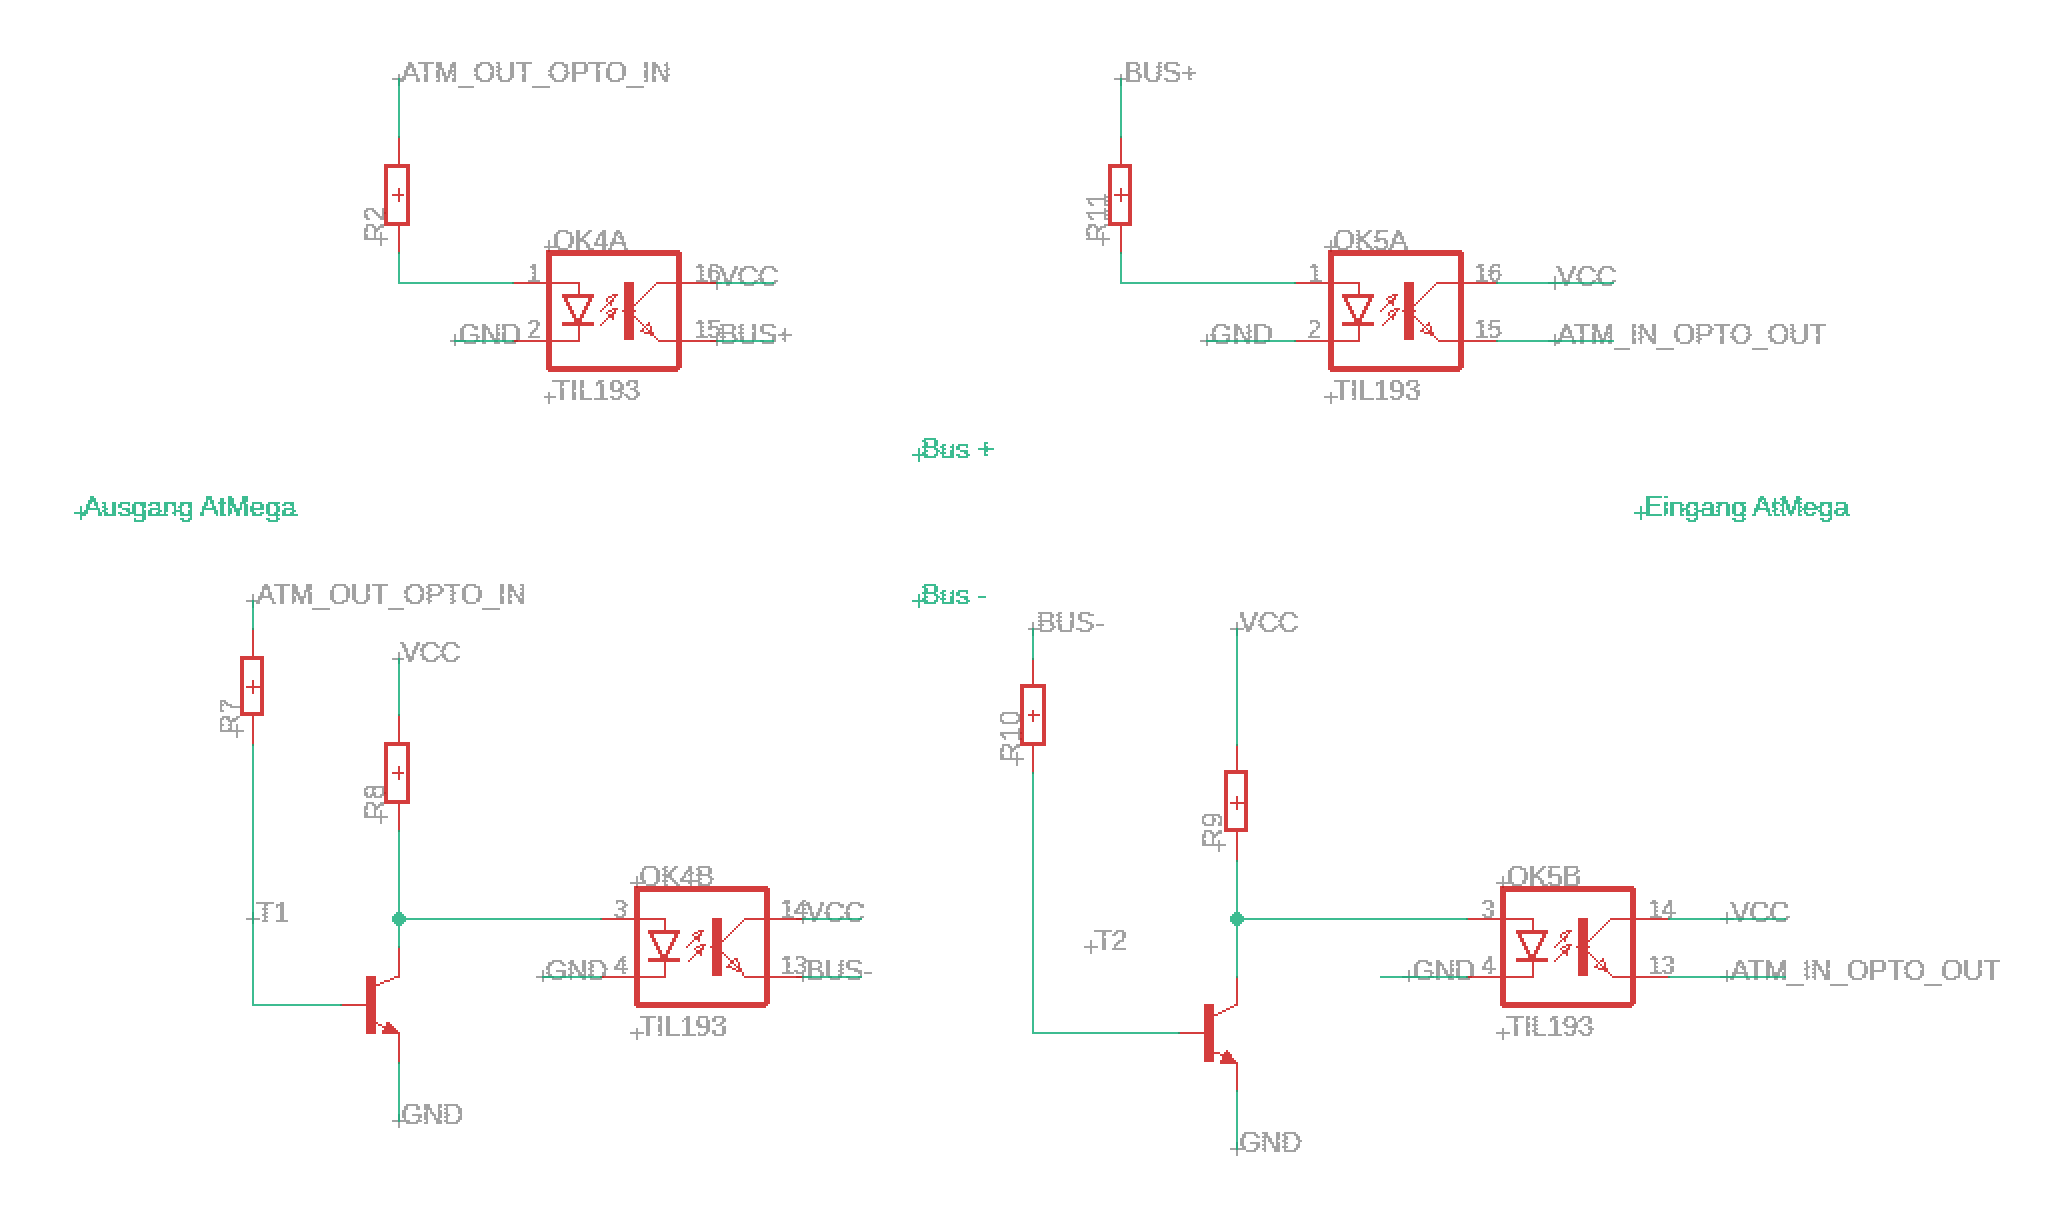
\includegraphics[width=1\textwidth]{Bilder/BU_Optokoppler.PNG}}
    \caption{Optokoppler Schaltung}
    \label{Optokoppler}
\end{figure}



\newpage
\section{Platine}
Beim Layout der Platine wurde auf die folgenden Punkte geachtet:

\begin{itemize}
	\item Platzierung der Kontaktstecker, entsprechend der modularen Verbindungsmöglichkeit
	\item Räumliche Nähe der zusammengehörenden Bauteile
	\item Optimierung der Masseführung durch Verwendung einer möglichst durchgehenden Massefläche
	\item Vermeidung von 90°-Ecken der Leiterbahnen, um Reflexionen zu minimieren
	\item Platzierung von Abblock- und Stützkondensator nahe den Versorgungspins der ICs.
\end{itemize}




\subsubsection{Differenzielle Übertragung}
Bei einem Layout für differenzielle Übertragung sollte zusätzlich auf die folgen Punkte geachtet werden:


\begin{itemize}
	\item Geringer Abstand zwischen den differenziellen Leitungen
	\item Gleiche Länge der differenziellen Leitungen
	\item Abstand zu anderen Leiterbahnen entsprechend Abb. \ref{AbstandLeiterbahnen}
	\item möglichst kurze Leitungen 
\end{itemize}


Wie in Abb. \ref{AbstandLeiterbahnen} vom Hersteller Empfohlen müssen die Leiterbahnen, von oben betrachtet zueinander einen möglichst geringen Abstand haben und zu anderen Leiterbahnen mindestens das Doppelte der Breite einer Leiterbahn. Diese Einstellungen kann beispielsweise in Eagle anhand der Signalnamen als Regel vorgenommen werden und werden dann automatisch eingehalten.

\subsection{Verbesserungen}
\subsubsection{Optimierung}

Da die erste Platine hauptsächlich zum Testen der differenziellen Übertragungsbauteile dient, sind einige Anpassungen geplant. \newline
Wenn die Inbetriebnahme wie erwartet gelingt und keine weiteren zu behebenden Fehler auftreten, soll vor allem Platz gespart werden, indem möglichst alle Bauteile durch SMD ersetzt werden. Die Jumper und Optokoppler sollen entfernt werden und es soll der Fokus auf Impedanzkontrolle gelegt werden, damit die differenzielle Übertragung gut funktioniert. \newline
Durch diese Änderungen wird die Platine voraussichtlich kleiner und günstiger werden. Ein Ziel ist es, das Tastatur-Modul auf die Maße des Controller-Moduls anzupassen, um die Modularität wie geplant möglichst ansprechend zu gestalten. \newline

Dafür soll von einer zwei Layer Platine auf vier Layer umgestiegen werden. Die Abstände der Signale zur Massefläche, wie in Formel \ref{Impedanz} zu sehen, einen Einfluss auf die Impedanz hat. Es gibt unterschiedliche Topologien zur Anordnung der Leiterbahnen auf den Layern der Platine.

\subsubsection{Kabelverbindung}
Außerdem soll als weitere Möglichkeit eine Kabelverbindung zwischen den Modulen entwickelt werden, um noch höhere Flexibilität zu ermöglichen.

\subsubsection{Anpassung der Layer}
Es soll von einer zwei Layer Platine auf vier Layer umgestiegen werden. Die Abstände der Signale zur Massefläche hat einen Einfluss auf die Impedanz, wie in \ref{Impedanz} zu sehen. Vom Hersteller wird ein vier Layer Stackup empfohlen, da sie die nötigen Spezifikationen für eine Impedanz von 100 Ohm ermöglichen. Es gibt unterschiedliche Topologien zur Anordnung der Leiterbahnen auf den Layern der Platine.

 
Bei einer Stripline-Topologie wie in Abb. \ref{Stripline} liegen die Leiterbahnen zwischen zwei Masseflächen eingebettet, was eine bessere Abschirmung bedeutet, aber auch eine höhere Kapazität. Daher wird vom Hersteller bei hochfrequenten Signalen eine Microstrip-Topologie, wie in Abb. \ref{MikrostripTopology} empfohlen.  


Außerdem wird die Breite und der Abstand der Leiterbahnen in der Software entsprechend der vom Hersteller angegebenen Werte für die Höhe und die Konstante des Dielektrikums, eingestellt. Bei dem von uns verwendeten Hersteller JLCPCB kann für die verschiedenen Dicken der Leiterplatte und entsprechend des verwendeten Dielektrikums die Dicke der einzelnen Layer eingesehen werden.  
In Formel \ref{Leiterbahnbreite} ist die Berechnung der Leiterbahnbreite mit Werten, die im Datenblatt der SN65LVDXXX Bauteile angegeben werden, entsprechend dem Terminationswiderstand von 100 Ohm.

\subsubsection{Anpassung der Leiterbahnbreite}
Außerdem wird die Breite und der Abstand der Leiterbahnen in der Software entsprechend der vom Hersteller angegebenen Werte für die Höhe und die Konstante des Dielektrikums, eingestellt. Bei dem von uns verwendeten Hersteller JLCPCB kann für die verschiedenen Dicken der Leiterplatte und entsprechend des verwendeten Dielektrikums die Dicke der einzelnen Layer eingesehen werden.
In Formel \ref{Leiterbahnbreite} ist die Berechnung der Leiterbahnbreite mit Werten, die im Datenblatt der SN65LVDXXX Bauteile angegeben werden, entsprechend dem Terminationswiderstand von 100 Ohm.

Eingesetzte Werte:
\begin{itemize}
	\item Dielektrizitätskonstante \( \varepsilon_r = 3.4 \)
	\item Abstand zwischen den differenziellen Leitungen \( S = 0.15 \, \text{mm} \)
	\item Dicke des Dielektrikums \( H = 0.18 \, \text{mm} \)
	\item Dicke der Leiterbahn \( T = 0.035 \, \text{mm} \)
	\item Zielimpedanz \( Z_0 = 100 \, \Omega \)
	\item Leiterbahnbreite \( W \) 
\end{itemize}



\begin{equation} \label{Impedanz}
	Z_{diff} = \frac{Z_0}{\sqrt{2}} \left( 1 + \frac{0.5}{\sqrt{1 + 4\cdot \frac{S}{W}}} \right)
\end{equation}


Berechnung der Leiterbahnbreite W mit den eingesetzten Werten:
\begin{equation} \label{Leiterbahnbreite}
W = \frac{5.98 \cdot 0.18}{\exp\left(\frac{100 \cdot \sqrt{3.4 + 1.41}}{87}\right)} - \frac{0.035}{0.8}
\end{equation}

\begin{equation} \label{Leiterbahnbreite}
	W = 0.043 \, \text{mm}
\end{equation}


\begin{figure}[H]
	\centering    
	\fbox{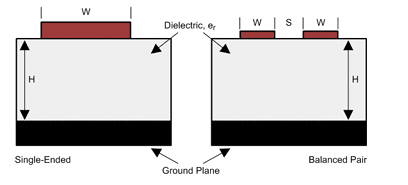
\includegraphics[width=0.85\textwidth]{Bilder/Mikrostrip.png}}
	\caption{Mikrostrip-Topology}
	\label{MikrostripTopology}
\end{figure}

\begin{figure}[H]
    \centering    
    \fbox{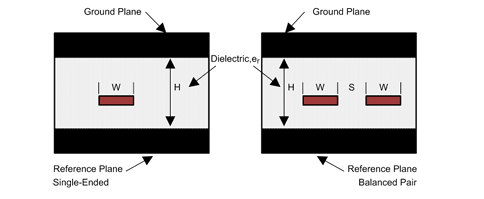
\includegraphics[width=0.85\textwidth]{Bilder/StriplineTopology.PNG}}
    \caption{Stripline-Topology}
    \label{Stripline}
\end{figure}

\begin{figure}[H]
    \centering    
    \fbox{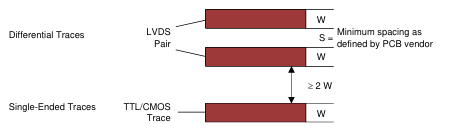
\includegraphics[width=0.85\textwidth]{Bilder/AbstandLeiterbahnen.png}}
    \caption{Abstand Leiterbahnen}
    \label{AbstandLeiterbahnen}
\end{figure}


\subsection{Layout}

In Abb. \ref{LayoutController} wird das Layout des Controllermoduls dargestellt.

In Abb. \ref{LayoutTastatur} wird das Layout des Keypadmoduls dargestellt. 

\begin{figure}[H]
	\centering    
	\fbox{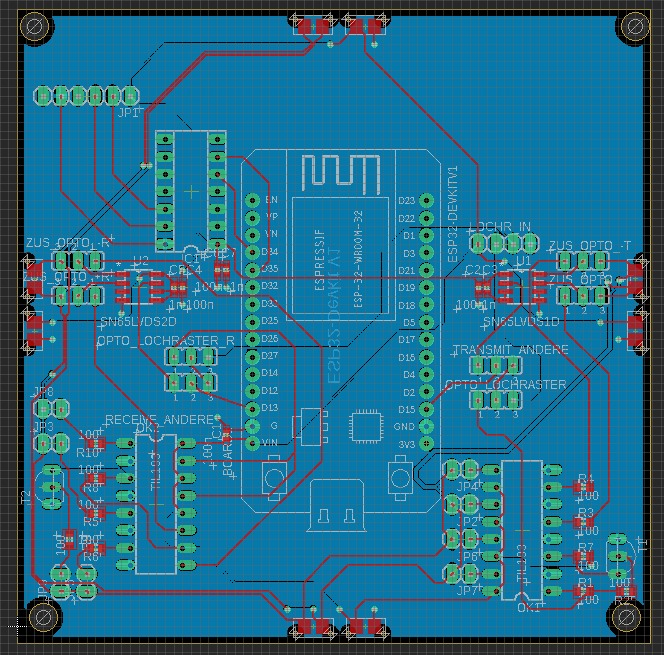
\includegraphics[width=0.85\textwidth]{Bilder/LayoutController.jpeg}}
	\caption{Layout Controller-Modul}
	\label{LayoutController}
\end{figure}

\begin{figure}[H]
	\centering    
	\fbox{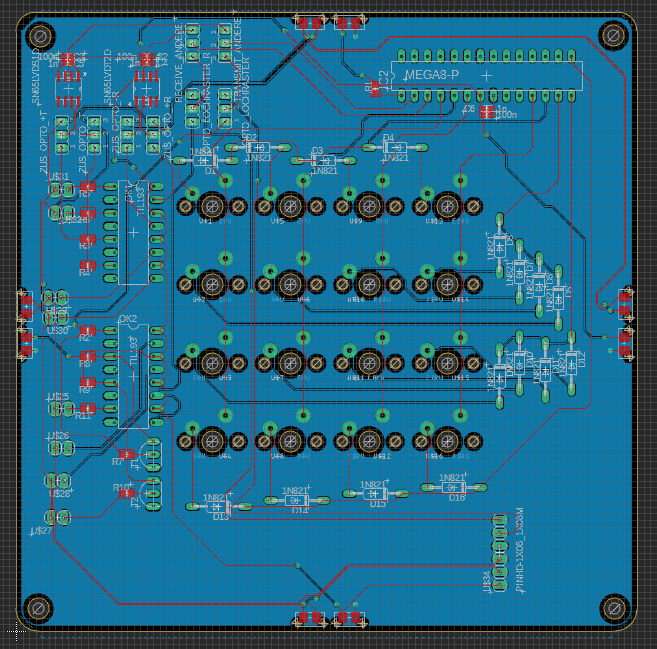
\includegraphics[width=0.85\textwidth]{Bilder/LayoutTastatur.png}}
	\caption{Layout Tastatur-Modul}
	\label{LayoutTastatur}
\end{figure}


